\documentclass[10pt,oneside]{article}

\usepackage{amsmath}
\usepackage{bm}
\usepackage{mathpazo}
\usepackage{graphicx}
\usepackage{enumerate}
\usepackage[x11names, svgnames]{xcolor} % for \definecolor

\usepackage[letterpaper]{geometry}
\geometry{verbose,tmargin=0.25in,bmargin=0.5in,lmargin=1in,rmargin=1.15in}

 \definecolor{saitPurple}{RGB}{112,40,119}
 \definecolor{statsMaroon}{rgb}{0.55, 0, 0}
 \definecolor{saitMaroon}{rgb}{0.55, 0, 0}
 \definecolor{saitRed}{RGB}{224,38,37}
 \definecolor{saitBlue}{rgb}{0, 0.59, 0.85}
 \definecolor{statsDeepBlue}{RGB}{0, 99, 167}
 \definecolor{saitDeepBlue}{RGB}{0, 99, 167}
 \definecolor{LightGrey}{RGB}{200,200,200}
%  \definecolor{boxBG}{RGB}{236, 227, 227}
%  \definecolor{boxBG}{RGB}{242, 233, 223}
\usepackage{xcolor}
\usepackage{cancel}
\usepackage{bm}
\usepackage{graphicx}
\usepackage{hyperref}
\usepackage{adjustbox}
\hypersetup{colorlinks, allcolors=.,urlcolor=structure}
\usepackage{booktabs}  % for top and bottom spacing in table cells, \addlinespace
\usepackage[x11names, svgnames]{xcolor} % for colors in handouts, auto loaded in Beamer?
\usepackage{tikz}
\usetikzlibrary{arrows.meta, math, calc, shadows,bending}
\usetikzlibrary{decorations.markings, decorations.fractals, decorations.text} % for chain, etc.
\usetikzlibrary{intersections}
\usepackage{pgfmath}
\usepackage{ifthen}
\usepgfmodule{oo}
\usetikzlibrary{shadings}
% \usetikzlibrary{decorations.shapes}
\usepackage[many]{tcolorbox}
\tcbuselibrary{skins} % for image boxes
\usepackage[absolute,overlay,showboxes]{textpos}
% \usepackage{textpos}
% \textblockorigin{0.0cm}{0.0cm}  %start all at upper left corner
\TPshowboxesfalse

\newcommand\lb{\linebreak}
\newcommand\Ra{\Rightarrow}
\newcommand\cd{\!\cdot\!}
\newcommand\x{\!\times\!}
\newcommand\pars{\par\smallskip}
\newcommand\parm{\par\medskip}
\newcommand\parb{\par\bigskip}
\renewcommand{\deg}{^\circ}

% counter for resuming enumerated list numbers
\newcounter{resumeenumi}
\newcommand{\suspend}{\setcounter{resumeenumi}{\theenumi}}
\newcommand{\resume}{\setcounter{enumi}{\theresumeenumi}}



% https://tex.stackexchange.com/questions/33703/extract-x-y-coordinate-of-an-arbitrary-point-in-tikz
\makeatletter
\providecommand{\gettikzxy}[3]{%
	\tikz@scan@one@point\pgfutil@firstofone#1\relax
	\edef#2{\the\pgf@x}%
	\edef#3{\the\pgf@y}%
}
\makeatother

\makeatletter
\newcommand{\verbatimfont}[1]{\def\verbatim@font{#1}}%
\makeatother

%%%%%%%%%%%%%%%%%%%%%%%%%%%%%%%%%%%%%%%%%%%%%%%%%%%%%%%%%%%%%%%%%%%%%%%%%%%%%%%%


% \newcommand{\tb}[4][0.8]{
% 	\begin{textblock*}{#1}(#2, #3)
% 		\raggedright
% 		#4
% 	\end{textblock*}
% }

% \def\tb

\newtcolorbox{statsbox}[2][] { 
  colback=white,
  colbacktitle=structure,
  colframe=structure,
  coltitle=white,  
  top=0.25cm,
	bottom=0.125cm,
	left=0mm,
	right=0mm,
  % fonttitle=\itshape\rmfamily,
  halign=flush left, 
  enhanced,
  drop fuzzy shadow,
  attach boxed title to top left={xshift=3.5mm, yshift=-2mm},
  title={#2}, #1}
\newtcolorbox{redbox}{colback=white, colframe=structure, enhanced, drop fuzzy shadow}
\newtcolorbox{titledbox}[1]{colback=white,colframe=structure,title={#1}}
\newtcbox{\tcb}[1][]{colback=white,boxsep=0pt,top=0.5cm,bottom=0.5cm,left=0.5cm,
		right=0.5cm, colframe=structure,  enhanced, drop fuzzy shadow, #1}
\newtcbox{\tcbfig}[1][1]{colback=white,boxsep=0pt,top=0.5cm,bottom=0.5cm,left=0.5cm,
		right=0.5cm, colframe=structure,  enhanced, drop fuzzy shadow, #1}
% tcb title
\newtcbox{\tcbt}[2][]{colback=white,boxsep=0pt,top=5pt,bottom=5pt,left=5pt,
		right=5pt, colframe=structure, enhanced, drop fuzzy shadow,  title={#2}, #1}
% tcb left title
\newtcbox{\tcbtl}[2][]{ colback=white,
  colbacktitle=structure,
  colframe=structure,
  coltitle=white,  
  top=0.25cm,
	bottom=0.125cm,
	left=0mm,
	right=0mm,
  % fonttitle=\bfseries,
  halign=flush left, 
  enhanced,
  drop fuzzy shadow,
  attach boxed title to top left={xshift=3.5mm, yshift=-2mm}, 
	title={#2}, #1}

\newtcbtheorem{myexam}{Example}%
{
	enhanced,
	colback=white,
	colframe=structure,
	% fonttitle=\bfseries,
	fonttitle=\itshape\rmfamily,
	drop fuzzy shadow,
	%description font=\mdseries\itshape,
	attach boxed title to top left={yshift=-2mm, xshift=5mm},
	colbacktitle=structure
	}{exam}% then \pageref{exer:theoexample} references the theo

% \newcommand{\myexample}[2][red]{
% 	% \tcb\tcbset{theostyle/.style={colframe=red,colbacktitle=yellow}}
% 	\begin{myexam}{}{}
% 		#2
% 	\end{myexam}
% 	% \tcbset{colframe=structure,colbacktitle=structure}
% }

\newtcbtheorem{myexer}{Exercise}%
{
	enhanced,
	colback=white,
	colframe=structure,
	% fonttitle=\bfseries,
	drop fuzzy shadow,
	fonttitle=\itshape\rmfamily,
	% description font=\mdseries\itshape,
	attach boxed title to top left={yshift=-2mm, xshift=5mm},
	colbacktitle=structure
	}{exer}



\newcommand{\mini}[2][0.8]{
	\begin{minipage}[c]{#1\columnwidth}
		\raggedright
		#2
	\end{minipage}
}
\newcommand{\minit}[2][0.8]{
	\begin{minipage}[t]{#1\columnwidth}
		% \raggedright
		#2
	\end{minipage}
}

% centered minipage with text \raggedright
%\cmini[width]{content}
\newcommand{\cmini}[2][0.8]{
	\begin{center}
		\begin{minipage}{#1\columnwidth}
			\raggedright
			#2
		\end{minipage}
	\end{center}
}

\newcommand{\fig}[2][1]{% scaled graphic
	\includegraphics[scale=#1]{#2}
}

% centred framed box black border
%\cbox[width]{content}
\newcommand{\cbox}[2][1]{% framed centered color box
	\setlength\fboxsep{5mm}
	\setlength\fboxrule{.2 mm}
	\begin{center}
		\fcolorbox{black}{white}{
			\vspace{-0.5cm}
			\begin{minipage}{#1\columnwidth}
				\raggedright
				#2
			\end{minipage}
		}
	\end{center}
	\setlength\fboxsep{0cm}
}

\newcommand{\ccbox}[4][1]{% framed centered color box
	\setlength\fboxsep{5mm}
	\setlength\fboxrule{.2 mm}
	\begin{center}
		\fcolorbox{#2}{#3}{
			% \vspace{-0.5cm}
			\begin{minipage}{#1\columnwidth}
				\vspace{-0.25cm}
				\raggedright				
				#4
				\vspace{-0.325cm}
			\end{minipage}
		}
	\end{center}
	\setlength\fboxsep{0cm}
}

\newcommand{\cfig}[2][1]{% centred, scaled graphic
	\begin{center}
		% \fcolorbox{structure}{white}{
		\tcbincludegraphics{
			\includegraphics[scale=#1]{#2}
		}
	\end{center}
}

% figure with tight border for photos
% \cfigb[saitMaroon]{borderwidth with unit}{scale}{image}
\newcommand{\stcsfig}[2][1]{
	% \usepackage{adjustbox}
	% \setlength{\fboxrule}{1pt}
	\begin{center}
		\tcbincludegraphics[width=#1\textwidth, boxrule=2pt, top=-3pt, right=-3pt, left=-3pt, bottom=-3pt,colframe=structure, sharp corners, enhanced, drop fuzzy shadow]{#2}
	\end{center}
}






% !TEX root = ../Beamer/statikz/statikz.tex

% \Channel[rotate=0]{coordinate}{draw}{fill}{scale}{lineWidth}
\newcommand{\Channel}[6][0]{
	\def\rotate{#1};
	\def\mid{#2}
	\def\lfill{#3}
	\def\lstroke{#4}
	\def\scale{#5};
	\def\lineWidth{#6};

	\begin{scope}[rounded corners=1pt, scale=\scale, rotate=\rotate]
		\filldraw[draw=\lstroke, fill=\lfill, line width=\lineWidth pt] ($(\mid) + (0,-3) $) -- ++(1.7,0) arc(0:85:0.25) -- ($ (\mid)+(0.4,-2.6) $) -- ($ (\mid)+(0.4,2.6) $) -- +(8.13:1.097)arc(-81.87:0:0.25) -- ($ (\mid)+(0,3) $)  -- cycle;
	\end{scope}
}

\newcommand{\Couple}[5][1]{
	\def\positive{#1};
	\def\lpin{#2}	
	\def\ldraw{#3}
	\def\diam{#4}
	\def\lwidth{#5}
	
	\begin{scope}[line cap = round]
		\ifthenelse{\equal{\positive}{1}}
			{
				\draw[line width=\lwidth mm, \ldraw, -{Latex[length=\lwidth*12, bend]}] ($ (\lpin)+(-150:\diam) $) arc (-150:165:\diam);
				% \draw[-latex, \ldraw, line width=\lwidth mm] ($ (\lpin)+(150:\diam) $) --+ (240:\lwidth/5);
			}
			{
				\draw[line width=\lwidth mm, \ldraw, -{Latex[length=\lwidth*12, bend]}] ($ (\lpin)+(150:\diam) $) arc (150:-165:\diam);
				% \draw[-latex, \ldraw, line width=\lwidth mm] ($ (\lpin)+(-140:\diam) $) --+ (120:\lwidth/5 );
			}
		
	\end{scope}
}
\newcommand{\DL}[9][1]{
  \def\forcedown{#1} % defaults to 1, force is downward
  \def\tl{#2} % top left, a coordinate
  \def\tr{#3} % top right. a coordinate
  \def\b{#4} % anywhere along the baseline (before any rotation), a coordinate 
  \def\lfill{#5} % background fill color
  \def\stroke{#6} % drawing color
  \def\spaces{#7} % number of spaces between arrows 
  \def\llinewidth{#8}
  \def\tiplength{#9}

  \gettikzxy{(\tl)}{\tlx}{\tly}
	\gettikzxy{(\tr)}{\trx}{\try}
	\gettikzxy{(\b)}{\bx}{\by}
  \pgfmathparse{abs(\try-\by)} \let\rlength\pgfmathresult
  \pgfmathparse{abs(\tly-\by)} \let\llength\pgfmathresult

  \fill[\lfill] (\tlx, \tly)--(\trx, \try)--(\trx, \by)--(\tlx, \by);
  \draw[\stroke, line cap = round, line width = \llinewidth mm] (\tl)--(\tr);
  
  % no empty lines in \tikzmath!
  \tikzmath{
    % Calculate the width of the load, and the spacing between arrows
    % Also, calculate the difference in length between adjacent arrows.
    \dx = \trx - \tlx; % width of dist load
    \dx = \dx / \spaces; % space between arrows
    \dy = \try - \tly; % difference between two load values
    \dy = \dy / \spaces; % difference between arrow-line lengths
    %    
    if \forcedown == 1 then {       
			for \i in {0,...,\spaces} {	
        \starty = \tly+\i*\dy;
        \length = \starty-\by;
        % in \tikzmath, drawing commands are enclosed in { }; 
        {
          \begin{scope}          
            \clip (\tlx,\tly) -- (\trx, \try) -- (\trx,\by) --(\tlx,\by);
            \draw[\stroke, line width = \llinewidth mm, -{Latex[length=\tiplength]}](\tlx+\i*\dx, \starty pt)-- +(270: \length pt);
          \end{scope}
        };
			};
    } else {
      for \i in {0,...,\spaces} {	
        \starty = \tly+\i*\dy;
        \length = \starty-\by;			
				{
          \begin{scope}          
            \clip (\tlx,\tly) -- (\trx, \try) -- (\trx,\by) --(\tlx,\by);
            \draw[\stroke, line width = \llinewidth mm, {Latex[length=\tiplength]}-](\tlx+\i*\dx, \starty pt)-- +(270: \length pt);
          \end{scope}          
        };
			};      
    };
    if \forcedown == 1 then {
      if \rlength > \tiplength then {
        {\draw[\stroke, line width = \llinewidth mm, -{Latex[length=\tiplength]}] (\trx, \try)--(\trx, \by);};
      } else {
         {\draw[\stroke, line width = \llinewidth mm] (\trx, \try)--(\trx, \by);};
      };    
      if \llength > \tiplength then {
        {\draw[\stroke, line width = \llinewidth mm, -{Latex[length=\tiplength]}] (\tlx, \tly)--(\tlx, \by);};
      } else {
        {\draw[\stroke, line width = \llinewidth mm] (\tlx, \tly)--(\tlx, \by);};
      };
    } else {
      if \rlength > \tiplength then {
        {\draw[\stroke, line width = \llinewidth mm, {Latex[length=\tiplength]}-] (\trx, \try)--(\trx, \by);};
      } else {
        {\draw[\stroke, line width = \llinewidth mm] (\trx, \try)--(\trx, \by);};
      };    
      if \llength > \tiplength then {
        {\draw[\stroke, line width = \llinewidth mm, {Latex[length=\tiplength]}-] (\tlx, \tly)--(\tlx, \by);};
      } else {
        {\draw[\stroke, line width = \llinewidth mm] (\tlx, \tly)--(\tlx, \by);};
      };
    };    
  } % \end tikzmath environment
} % end of \DL definition
%\Member{startpt}{endpt}{outer fill color}{inner fill color}{stroke}{height}{radius}{linewidth}
\providecommand{\Member}[8]{
  % name the points
  \coordinate(start) at (#1);
  \coordinate(end) at (#2);
  \edef\ofill{#3}%
  \edef\ifill{#4}%
  \edef\stroke{#5}%
  \edef\height{#6} % cm
  \edef\radius{#7} % cm
  \edef\linewidth{#8} % mm

  \coordinate(delta) at ($ (end)-(start) $);
  \gettikzxy{(delta)}{\dx}{\dy}
  \gettikzxy{(start)}{\sx}{\sy}
  \pgfmathparse{veclen(\dx, \dy)} \let\length\pgfmathresult

  \pgfmathparse{\dx==0}%
  % \ifnum low-level TeX for integers
  \ifnum\pgfmathresult=1 % \dx == 0
    \pgfmathsetmacro{\rot}{\dy > 0 ? 90 : -90}
  \else
    \pgfmathsetmacro{\rot}{\dx > 0 ? atan(\dy / \dx) : 180 + atan(\dy / \dx)}
  \fi

  
   
  \shadedraw[transform canvas = { rotate around = {\rot:(\sx,\sy)}}, line width = \linewidth, rounded corners = \radius mm, top color = \ofill, bottom color = \ofill, middle color = \ifill, draw = \stroke] ($ (start)+(-0.5*\height, 0.5*\height) $) -- ++(\height cm +\length pt, 0 ) -- ++(0, -\height) -- ++ (-\height cm -\length pt, 0) -- cycle;


  \shadedraw[ball color = \ofill!50!\ifill, draw = \stroke] (start) circle (\height/8);
  \shadedraw[ball color = \ofill!50!\ifill, draw = \stroke] (end) circle (\height/8);
  %  \pgfresetboundingbox

  
  


}

%\Member{startpt}{endpt}{outer fill color}{inner fill color}{stroke}{height}{radius}{linewidth}
\providecommand{\Meme}[8]{
  \coordinate(start) at (#1);
  \coordinate(end) at (#2);
  \edef\ofill{#3}%
  \edef\ifill{#4}%
  \edef\stroke{#5}%
  \edef\height{#6} % cm
  \edef\radius{#7} % cm, should be half \height or less
  \edef\linewidth{#8} % mm

  


  \coordinate(delta) at ($ (end)-(start) $);
  \gettikzxy{(delta)}{\dx}{\dy}
  \gettikzxy{(start)}{\sx}{\sy}
  \gettikzxy{(end)}{\ex}{\ey}
  \pgfmathparse{veclen(\dx, \dy)} \let\length\pgfmathresult
  \pgfmathparse{\height*28.435} \let\heightpt\pgfmathresult
  \pgfmathparse{\heightpt/\length} \let\ratio\pgfmathresult
  \pgfmathparse{1/\ratio} \let\inverse\pgfmathresult
  

  \pgfmathparse{\dx==0}%
  % \ifnum low-level TeX for integers
  \ifnum\pgfmathresult=1 % \dx == 0
    \pgfmathsetmacro{\rot}{\dy > 0 ? 90 : -90}
  \else
    \pgfmathsetmacro{\rot}{\dx > 0 ? atan(\dy / \dx) : 180 + atan(\dy / \dx)}
  \fi

  \pgfmathparse{round(mod(abs(\rot),90))} \let\tmp\pgfmathresult
  \pgfmathsetmacro{\rotmod}{\tmp>45?90-\tmp:\tmp}
  \pgfmathparse{(0.007*\rotmod-0.315)/45+1.017} \let\rotfudge\pgfmathresult

  % \pgfmathparse{mod(abs(\rot),90)} \let\moded\pgfmathresult
  % \ifthenelse{\moded>45}{
  %   \pgfmathparse{90-\moded} \let\rotmod\pgfmathresult    
  % }{
  %   \pgfmathparse{div(\moded,1)} \let\rotmod\pgfmathresult   
  % }


  
  \pgfmathparse{1+3.62/(1+(\inverse/0.714)^1.69)} \let\fudge\pgfmathresult
  \pgfmathparse{50*(1-\ratio)*\fudge*\rotfudge} \let\colorstop\pgfmathresult
  \pgfmathparse{(100-\colorstop)} \let\colorstoptwo\pgfmathresult

  \pgfdeclareverticalshading{myshade}{100bp}{%
					color(0bp)=(\ofill);
					% color(\colorstop bp)=(\ofill);
					color(\colorstop bp)=(\ofill);
					color(50 bp)=(\ifill);
					color(\colorstoptwo bp)=(\ofill);
					color(100bp)=(\ofill)}

  % \tikzset{shading=myshade}

  \begin{scope}[rotate around = {\rot:(start)}, rounded corners = \radius cm, shading angle=\rot]
    \begin{scope} 
      \path[clip]($ (start)+(-0.5*\height, 0.5*\height cm) $) rectangle +(\length pt+\height cm, -\height);
      \shade[shading=myshade] ($ (start)+(-0.5*\height, 0.5*\length pt) $) rectangle +(\length pt+\height cm, -\length pt);
    \end{scope}
  \draw[line width=\linewidth, \stroke] ($ (start)+(-0.5*\height, 0.5*\height cm) $) rectangle +(\length pt+\height cm, -\height);

  % \shadedraw[top color=\ofill, bottom color=\ofill, middle color=\ifill, rotate around = {\rot:(start)}, draw=\stroke, rounded corners = \radius cm, , shading angle=\rot] ($ (start)+(-0.5*\height cm, 0.5*\length pt) $) rectangle +(\length pt+\height cm, -\length pt);
  \end{scope}

  % \pgfresetboundingbox


  % \node[orange] at (0,-1) {rot: \rot};  
  % \node[orange] at (0,-1.5) {rotmod: \rotmod};  
  % \node[orange] at (0,-2) {rotfudge: \rotfudge};  
  % \node[orange] at (-2,-1) {stop2: \colorstoptwo};  
  % \node[orange] at (-2,-1.5) {l/h: \inverse};  
  % \node[orange] at (-2,-2) {fudge: \fudge};  

 
  
  \shade[ball color=\ofill] (start) circle (\height/4);
  \shade[ball color=\ofill] (end) circle (\height/4);

  % \draw(current bounding box.south west) rectangle (current bounding box.north east);


}

\newcommand{\PC}[6][0]{%
  \edef\lrotate{#1}%
  \edef\lpin{#2}%
  \edef\lfill{#3}%
  \edef\ldraw{#4}%
  \edef\lscale{#5}%
  \edef\lwidth{#6}%
  \edef\h{1}%
  \edef\r{0.3}%
  \begin{scope}[scale=\lscale, rotate=\lrotate]
	\filldraw[draw=\ldraw, fill=\lfill, line width=\lwidth mm] ($ (\lpin) + (0.201*\h+1.0353*\r ,-0.75*\h) $) -- ++(105: 0.77646*\h+0.26795*\r) arc (15:165:\r) -- ++(-105:0.77646*\h+0.26795*\r) -- cycle;

	\shadedraw[ball color=\lfill, draw=\ldraw, line width = \lwidth mm] (\lpin) circle (1.5mm);

	\filldraw[rounded corners=\lscale pt, draw=\ldraw, fill=\lfill, line width=\lwidth mm] ($ (\lpin) - (1,1) $) rectangle +(2,0.25);
  \end{scope}%
}



% !TEX root = ../../Beamer/statikz/statikz.tex


\newcommand{\EyeConnection}[6][0]{
	\def\lrotate{#1};
	\def\lpin{#2}
	\def\lfill{#3}
	\def\ldraw{#4}
	\def\lscale{#5}
	\def\lwidth{#6}
	\def\h{1}
	\def\r{0.3}
	\begin{scope}[scale=\lscale, rotate=\lrotate]
		\filldraw[draw=\ldraw, fill=\lfill, line width=\lwidth pt] ($(\lpin) + (0.201*\h+1.0353*\r ,-0.75*\h)$) -- ++(105: 0.77646*\h+0.26795*\r) arc (15:165:\r) -- ++(-105:0.77646*\h+0.26795*\r) -- cycle;

		\fill[outer color=\lfill, middle color=red, inner color=black, line width = \lwidth pt] (\lpin) circle (2.5mm);
		\filldraw[fill=white, draw=\ldraw, line width = \lwidth pt] (\lpin) circle (1.25mm);

		\filldraw[rounded corners=\lscale pt, draw=\ldraw, fill=\lfill, line width=\lwidth pt] ($ (\lpin) - (1,1) $) rectangle +(2,0.25);
	\end{scope}
}

% !TEX root = ../Beamer/02ForceVectors/02ForceVectors.tex


\newcommand{\EyeBolt}[6][0]{
	\def\lrotate{#1};
	\def\lpin{#2}
	\def\lfill{#3}
	\def\ldraw{#4}
	\def\lscale{#5}
	\def\lwidth{#6}
	%\def\h{1.5}
	\def\r{0.3}
	\begin{scope}[scale=\lscale, rotate=\lrotate]
		\filldraw[draw=\ldraw, fill=\lfill, line width=\lwidth pt] ($(\lpin) + (-0.7,-1.25)$) arc(180:90:.2) -- ++(0.05,0)arc(-90:0:0.2) -- ++(0.05,0.65)arc(225:-45:0.28284)-- ++(0.05,-.65)arc(180:270:.2)-- ++(0.05,0)arc(90:0:0.2) -- cycle;
		\fill[outer color=\lfill, inner color=black, line width = 0] (\lpin) circle (2.25mm);
		\filldraw[fill=white, draw=\ldraw, line width = \lwidth pt] (\lpin) circle (1.25mm);

		\begin{scope}[even odd rule]
			\fill[\lfill] (\lpin) circle (2.5mm)
			(\lpin) circle (2.125mm);
		\end{scope}

		\filldraw[rounded corners=\lscale pt, draw=\ldraw, fill=\lfill, line width=\lwidth pt] ($ (\lpin) - (1,1.5) $) rectangle +(2,0.25);
	\end{scope}
}

\input{../../includes/Skywalker.tex}

\newcommand{\PulleyC}[8][0]{
	\def\rotate{#1};
	\def\pin{#2}
	\def\lfill{#3}
	\def\ldraw{#4}
	\def\len{#5}
	\def\wid{#6}
	\def\lscale{#7};
	\def\lwidth{#8};
	\def\h{1}
	\def\r{0.35}
	\def\rr{0.675}
	\begin{scope}[scale=\lscale, rotate=\rotate]

		
		
		\filldraw[draw=\ldraw, fill=\lfill, line width=\lwidth mm] (\pin) circle (\h*\rr cm);
		
		\filldraw[draw=\ldraw, fill=\lfill!70!black, line width=\lwidth mm] (\pin) circle (\h*\rr*0.75 cm);

		\filldraw[ draw=\ldraw, fill=\lfill, line width = \lwidth mm] ($(\pin) + (-\wid,0) $) arc(180:0:\wid) -- ++(0,-\len) arc(0:-180:\wid) -- cycle;		

		% \shadedraw[fill=\lfill, line width = \lwidth pt, draw=\lfill!80!black] (\pin) circle (\h mm);
		\shadedraw[ball color=\lfill, draw=\ldraw, line width = \lwidth mm] (\pin) circle (2*\h*\rr mm);
		\shadedraw[ball color=\lfill, draw=\ldraw, line width = \lwidth mm] ($ (\pin)+(0,-\len) $) circle (2*\h*\rr mm);

		
	\end{scope}
}

% !TEX root = ../Beamer/statikz/statikz.tex

% \Pulley[rotation]{A}{wheel color}{support color}{scale}{line width}
\newcommand{\Pulley}[6][0]{
	\def\lrotate{#1};
	\def\lpin{#2}
	\def\lfill{#3}
	\def\ldraw{#4}
	\def\lscale{#5}
	\def\lwidth{#6}
	\def\h{1}
	\def\r{0.3}
	\def\rr{0.5}
	\begin{scope}[scale=\lscale, rotate=\lrotate]

		\filldraw[draw=\ldraw, fill=\lfill, line width=\lwidth mm] (\lpin) circle (\h*\rr cm);

		\filldraw[draw=\ldraw, fill=\lfill, line width=\lwidth mm] ($(\lpin) + (0.201*\h+1.0353*\r ,-0.75*\h)$) -- ++(105: 0.77646*\h+0.26795*\r) arc (15:165:\r) -- ++(-105:0.77646*\h+0.26795*\r) -- cycle;

		\shadedraw[ball color=\lfill, draw=\ldraw, line width = \lwidth mm] (\lpin) circle (2*\h*\rr mm);

		\filldraw[rounded corners=\lscale pt, draw=\ldraw, fill=\lfill, line width=\lwidth mm] ($ (\lpin) - (1,1) $) rectangle +(2,0.25);
	\end{scope}
}

% !TEX root = ../Beamer/statikz/statikz.tex

% \Ring{A}{outer color}{inner color}{outer radius}{inner radius}{line width}
\newcommand{\Ring}[6]{
	\def\lpin{#1}
	\def\lfill{#2}
	\def\ldraw{#3}
	\def\outerr{#4}
	\def\innerr{#5}
	\def\lwidth{#6}

	\begin{scope}

		\makeatletter
		\providecommand{\gettikzxy}[3]{%
			\tikz@scan@one@point\pgfutil@firstofone#1\relax
			\edef#2{\the\pgf@x}%
			\edef#3{\the\pgf@y}%
		}
		\makeatother

		\gettikzxy{(\lpin)}{\cx}{\cy}
		\pgfdeclareradialshading{ring}{\pgfpoint{0cm}{0cm}}
		{
			color(0cm)=(black);
			color(0.5cm)=(\lfill);
			color(.65cm)=(\ldraw);
			color(1cm)=(\lfill)
		}
		% \pgfuseshading{ring}



	\end{scope}


\begin{scope}[even odd rule]
	% \draw (\lpin) circle (\innerr);
	\filldraw[shading=ring, fill=\lfill, draw=\ldraw, line width=\lwidth] (\lpin) circle (\outerr cm)
		(\lpin) circle (\innerr);
		\draw[black, line width = \lwidth mm] (\lpin) circle (\innerr cm);
		\draw[black, line width = \lwidth mm] (\lpin) circle (\outerr cm);
\end{scope}


}



%\Rocker[rotate=0]{coordinate}{draw}{fill}{scale}{line width}
\newcommand{\Rocker}[6][0]{%
	\edef\rotate{#1}%
	\edef\pin{#2}%
	\edef\lfill{#3}%
	\edef\ldraw{#4}%
	\edef\lScale{#5}%
	\edef\lwidth{#6}%
	\edef\h{1}%
	\edef\r{0.3}%

	\begin{scope}[scale=\lScale, rotate=\rotate]

		\filldraw[draw=\ldraw, fill=\lfill, line width = \lwidth mm] ($(\pin) + (0,-\h)$)arc(-90:-57.54:\h) -- ++(105:0.95394)arc(15:165:\r) -- ++(-105:0.95394)arc(-122.458:-90:\h);

		\shadedraw[ball color=\lfill, \ldraw, line width = \lwidth pt] (\pin) circle (1.5mm);
	\end{scope}
}

% !TEX root = ../Beamer/statikz/statikz.tex

% \WBeam[rotate=0]{coordinate}{draw}{fill}{scale}{line width}
\providecommand{\WBeam}[6][0]{
	\def\lrotate{#1}
	\def\lcentroid{#2}
	\def\lfill{#3}
	\def\ldraw{#4}
	\def\lscale{#5}
	\def\llineWidth{#6}

	\begin{scope}[rounded corners=1pt, scale=\lscale, rotate=\lrotate]
		\filldraw[draw=\ldraw, fill=\lfill, line width=\llineWidth pt] ($(\lcentroid) + (-2,-3) $) -- ++(4,0) -- ++(0,0.5) -- ++(-1.85,0) -- ++(0,5) -- ++(1.85,0) -- ++(0,0.5) -- ++(-4,0) -- ++(0,-0.5) -- ++(1.85,0) -- ++(0,-5) -- ++(-1.85, 0) -- cycle;
	\end{scope}
}


% https://tex.stackexchange.com/questions/731957/how-to-supress-missing-character-there-is-no-u003b-in-font-nullfont
\tracinglostchars=1

\hfuzz=150pt
\setlength{\parindent}{0pt}
\def\scale{1}

\begin{document}

%%%%%%%%%%%%%%%%%%%%%%%%%%%%%%%%%%%%%%%%%%%%%%%%%%%%%%%%%%%%%%%%%%%%%%%%%%%%%%%%%%%%%%%%%%%%%%%%%%%%
% page 1
%%%%%%%%%%%%%%%%%%%%%%%%%%%%%%%%%%%%%%%%%%%%%%%%%%%%%%%%%%%%%%%%%%%%%%%%%%%%%%%%%%%%%%%%%%%%%%%%%%%%
\begin{textblock*}{1.0\textwidth}(1in, 0.25in)
	
\begin{tikzpicture}[line width= 0.3mm, scale=1.0525]
		\draw[ color=gray!50, step=0.25in] (0,0) grid (7in,10in);
	\end{tikzpicture}
\end{textblock*}


\begin{textblock*}{6.88in}(1in, 0.1in)
  \cbox{
    \centering\huge
    \textbf{Engineering Statics - 05 Moments}
  }
\end{textblock*}

\begin{textblock*}{3in}(1in, 1in)
	\cbox{
		\underbar{\bf Example 1:} Determine the moment, $M_A$, of the $3.5$ kN force applied at $B$, about the point $A$.
	}
\end{textblock*}
\begin{textblock*}{3.35in}(4.525in, 1in)
	\cbox{
		\centering
			\def\scale{0.8}
			% !TEX root = ../../Beamer/statikz/statikz.tex


\tikz[scale=\scale]{


	\coordinate (A) at (0,0);
	\coordinate (B) at (-2,5);

	\draw[very thick]  ($ (A)-(4,0) $) -- ($ (A)+(2,0) $);
	\Meme{A}{B}{Gray!50}{Gray!50}{black}{0.5}{0.125}{0.5}
	\fill[Gray!50] ($ (A)-(4,0) $) rectangle ($ (A)+(2,-1) $);

	\fill[black] (B) circle (2pt) node[left, outer sep=1.5mm, black] {$\bm B$};
	\fill[black] (A) circle (2pt) node[below, black] {$\bm A$};

	\draw[ultra thick, -latex] (B) -- +(-120:3) node[above left]{$3.50\,$kN};
	\draw ($ (A)+(21.8:0.5) $) -- +(21.8:1);
	\draw ($ (B)+(21.8:0.5) $) -- +(21.8:1);
	\draw[latex-latex] ($ (A)+(21.8:1) $) -- node[sloped, fill=white]{$2.30\,$m} ($ (B)+(21.8:1) $);
	\draw ($ (B)+(-68.2:1.75)  $) -- ($ (B)+(-68.2:2.75)  $);
	\draw[latex-latex] ($ (B)+(-68.2:2.2)  $) arc (-68.2:-120:2.2);
	\node[fill=white, inner sep = 0.2mm] at ($ (B)+(-95:2.15) $){\small $51.8^\circ$};

  % \path[name path=AC] (A)--(150:4.75);
  % \path[draw, name path=BC] (B) -- +(-120:3.75) ;
  % \path[name intersections={of=AC and BC, by={C}}] ;
  % \draw (A)--(C) node[midway, fill=white] {$ d $};
  % \draw ($ (C)+(60:0.325) $) --++(-30:0.325) --+(-120:0.325);

}

	}
\end{textblock*}


\begin{textblock*}{3.5in}(1in, 5.5in)
	\cbox{
		\underbar{\bf Example 2:} Determine the sum of the moments of the forces, acting at $B$ and $C$, about the point $A$. \parm  Also, sum the moments of the forces about the point $B$.
	}
\end{textblock*}
\begin{textblock*}{2.85in}(5.025in, 5.5in)
	\cbox{
		\centering
		\def\scale{0.8}
		% !TEX root = ../../Beamer/statikz/statikz.tex


\tikz[scale=\scale]{
	\small
	\def\hi{0.2}


	\def\extend{0.5}

	\coordinate (A) at (0,0);
	\coordinate (B) at (4,0);
	\coordinate (C) at (4,2);

	\filldraw[fill=Gray!50, draw=black, thick, rounded corners=1mm] ($ (A)+(-1,4) $) -- ++(1,0) -- ++(0,-3.65) -- ($ (B)+(-0.35,0.35) $) -- ($ (C)+(-0.35,0.5) $)  -- ($ (C)+(0.35,0.5) $) -- ($ (B)+(0.35,-0.35) $)-- ($ (A)+(0,-0.35)  $)--++(0,-2)--+(-1,0);

	\draw[ultra thick, -latex, name path=BD] (B) -- +(131:3.75) node[above] {$2.30\,$kN};
	\draw[ultra thick, -latex, line cap=round] (C) -- +(90:1.5) node[above, black] {$2.05\,$kN};
	\draw[ultra thick, -latex, line cap=round] (C) -- +(0:1.75) node[above, black] {$2.84\,$kN};
	\draw ($ (B)-(1.5,0) $) -- ($ (B)-(2.5,0) $);
	\draw ($ (C)+(1,0) $) -- +(1:0);

	\draw[latex-latex] ($ (B)+(131:2)  $) arc (131:180:2);

	\fill[black] (A) circle (2pt) node[left] {$\bm A$};
	\fill[black] (B) circle (2pt) node[below right, outer sep=2mm] {$\bm B$};
	\fill[black] (C) circle (2pt) node[xshift=0.25mm, above right, outer sep=2mm] {$\bm C$};
	\node[fill=white] at ($ (B)+(155:2) $){$49^\circ$};
	\draw ($ (B)+(0.5,0) $) -- +(1,0);
	\draw ($ (B)+(0,-0.5) $) -- +(0,-1);
	\draw[latex-latex] ($ (A)-(0,1) $) -- node[fill=white] {$4.00\,$m} ($ (B)-(0,1) $);
	\draw[latex-latex] ($ (C)+(1,0) $) -- node[fill=white, xshift=0.25cm] {$2.00\,$m} ($ (B)+(1,0) $);

  % \path[name path=AD] (A)--+(41:4);
  % \path[name intersections={of=AD and BD, by={D}}] ;
  % \draw (A)--(D)node[midway, fill=white] {$ d $};
  % \draw ($ (D)+(131:0.325) $) --++(221:0.325)--+(-49:0.325);

}

	}
\end{textblock*}


%%%%%%%%%%%%%%%%%%%%%%%%%%%%%%%%%%%%%%%%%%%%%%%%%%%%%%%%%%%%%%%%%%%%%%%%%%%%%%%%%%%%%%%%%%%%%%%%%%%
% page 2
%%%%%%%%%%%%%%%%%%%%%%%%%%%%%%%%%%%%%%%%%%%%%%%%%%%%%%%%%%%%%%%%%%%%%%%%%%%%%%%%%%%%%%%%%%%%%%%%%%%
~\newpage
\begin{textblock*}{1.0\textwidth}(1in, 0.25in)
	
\begin{tikzpicture}[line width= 0.3mm, scale=1.0525]
		\draw[ color=gray!50, step=0.25in] (0,0) grid (7in,10in);
	\end{tikzpicture}
\end{textblock*}


\begin{textblock*}{2.5in}(1in, 0.1in)
	\cbox{
			\underbar{\bf Exercise 1:} Rigid beam $ABCD$ is supported at $A$ and at $D$, and is subjected to the two forces shown at $B$ and $C$.\parm
			Determine the value of the reaction at $D$, $R_D$, if the sum of the moments about $A$, $\Sigma M_A$, is zero and the reaction at $D$ is vertically upwards.
	}
\end{textblock*}
\begin{textblock*}{3.85in}(4.025in, 0.1in)
	\cbox{
		\centering
		\def\scale{0.65}
		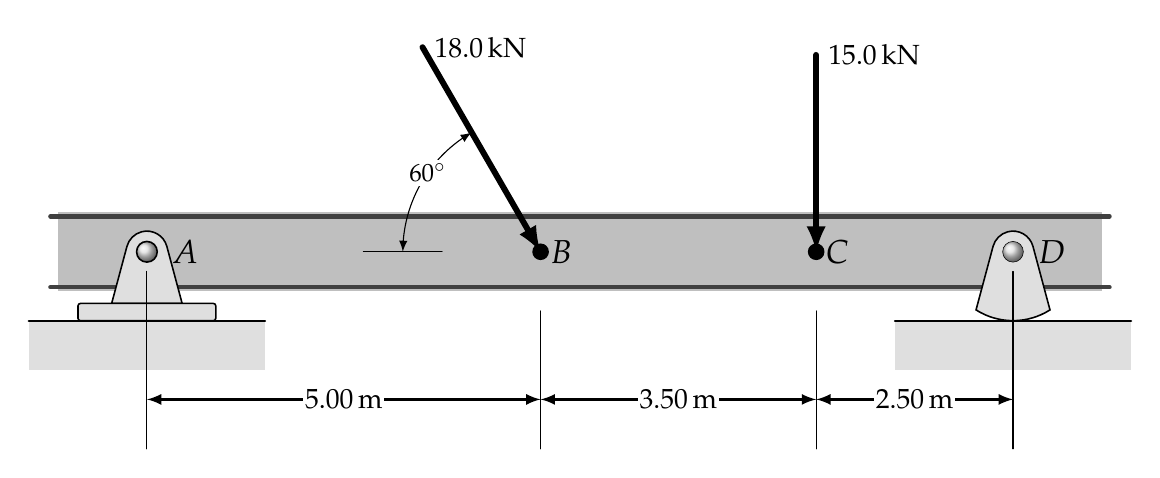
\begin{tikzpicture}[scale=\scale, line cap=round]
	\def\thickness{thick}
	\def\stroke{black}
	\def\hi{.4}
	\def\radii{0}
	\def\extend{3*\hi}
	\def\nuhi{0.45}
	\def\nuext{1.225}

	\coordinate (A) at (0, 0);
	\coordinate (B) at (5, 0);
	\coordinate (C) at (8.5, 0);
	\coordinate (D) at (11, 0);

	\fill[Gray!50] ($ (A)+(-1.125,0.5) $) rectangle ($ (D)+(1.125,-0.5) $);

	\fill[Gray!25] ($ (A)-(1.5,0.875) $) rectangle ($ (A)+(1.5,-1.5) $);
	\fill[Gray!25] ($ (D)-(1.5,0.875) $) rectangle ($ (D)+(1.5,-1.5) $);
	\draw[thick] ($ (A)-(1.5,0.875) $) -- ($ (A)+(1.5,-0.875) $);
	\draw[thick] ($ (D)-(1.5,0.875) $) -- ($ (D)+(1.5,-0.875) $);

	\draw[ultra thick, Gray!50!black] ($ (A)+(-\nuext, \nuhi) $) -- ($ (D)+(\nuext, \nuhi) $);
	\draw[ultra thick, Gray!50!black] ($ (A)+(-\nuext, -\nuhi) $) -- ($ (D)+(\nuext, -\nuhi) $);
	

	\fill[black] (A) circle (3pt) node[xshift=1mm, right, outer sep=1mm] {\large $A$};
	\fill[black] (B) circle (3pt) node[right] {\large $B$};
	\fill[black] (C) circle (3pt) node[right] {\large $C$};
	\fill[black] (D) circle (3pt) node[xshift=1mm,right, outer sep=1mm] {\large $D$};

	\PC{A}{Gray!25}{black}{0.875}{0.2}
	\Rocker{D}{Gray!25}{black}{0.875}{0.2}


	\draw ($ (B)+(0,-0.75) $) -- +(0,-1.752);
	\draw ($ (A)+(0,-0.25) $) -- +(0,-2.252);
	\draw ($ (C)+(0,-0.75) $) -- +(0,-1.752);
	\draw ($ (D)+(0,-0.25) $) -- +(0,-2.252);

	\draw[thick, latex-latex] ([yshift=-1.875cm]A) -- node[fill=white, inner sep= 0.2mm]{$5.00\,$m}([yshift=-1.875cm]B);
	\draw[thick, latex-latex] ([yshift=-1.875cm]B) -- node[fill=white, inner sep= 0.2mm]{$3.50\,$m}([yshift=-1.875cm]C);
	\draw[thick, latex-latex] ([yshift=-1.875cm]C) -- node[fill=white, inner sep= 0.2mm]{$2.50\,$m}([yshift=-1.875cm]D);

	\draw ($ (B)-(1.25,0) $) -- +(-1,0);

	\draw[line width=0.75mm,  latex-] (C) -- +(0,2.5) node[right] { $15.0\,$kN};
	\draw[line width=0.75mm,  latex-] (B) -- ($ (B) + (120:3) $) node[right] {$18.0\,$kN};

	\draw[latex-latex] ($ (B)+(180:1.75)  $)  arc (180:120:1.75);
	\path ($ (B)+(145:1.75) $) node[fill=white, inner sep=0.5mm] {\small $60\deg$};

  
  

\end{tikzpicture}

	}
\end{textblock*}



\begin{textblock*}{3.25in}(1in, 7in)
	\cbox{
		\underbar{\bf Example 3:}\parm
		Determine the moment about $A$ of the force applied to $B$ by resolving the force at $B$ into horizontal and vertical components.
	}
\end{textblock*}
\begin{textblock*}{3.125in}(4.775in, 7in)
	\cbox{
	\centering
	\tikz[scale=\scale]{

	\coordinate (A) at (0,0);
	\coordinate (B) at (5,0);

  \fill[gray!50, rounded corners=5mm] ($ (A)+(0,1.5) $) to [out=225, in=135] ($ (A)-(0,1.5) $);
  % \fill[Sienna3] (($ (A)+(0,1) $) rectangle ($ (A)+(0,-3) $);)
  \draw[semithick] ($ (A)+(0,1.5) $) -- ($ (A)+(0,-1.5) $);
  \Meme{A}{B}{gray!50}{gray!30}{black}{0.5}{0}{0.1}
  \draw[line width= 0.5mm, line cap=round] ($ (A)+(-0.25,0.25) $) --  ($ (B)+(0.25,0.25) $);
  \draw[line width= 0.5mm, line cap=round] ($ (A)+(-0.25,-0.25) $) --  ($ (B)+(0.25,-0.25) $);

  \draw[ultra thick, -latex] (B) -- +(-63:2) node[below] {$3.00\,$kN};
  \fill (A) circle (2pt) node[right] {$A$};
  \fill (B) circle (2pt) node[left] {$B$};

  \draw ($ (B)+(0,0.5) $) -- +(0,0.5);
  \draw[latex-latex] ($ (A)+(0,0.75) $) -- node[midway, fill=white] {$3.00\,$m} ($ (B)+(0,0.75) $);
  \draw ($ (B)+(0.5,0) $) -- +(1,0);
  \draw[latex-latex] ($ (B)+(1,0) $)  arc(0:-63:1) node[midway, fill=white, inner sep=0.3mm] {$63\deg$};
}

	}
\end{textblock*}




%%%%%%%%%%%%%%%%%%%%%%%%%%%%%%%%%%%%%%%%%%%%%%%%%%%%%%%%%%%%%%%%%%%%%%%%%%%%%%%%%%%%%%%%%%%%%%%%%%%%
% page 3 
%%%%%%%%%%%%%%%%%%%%%%%%%%%%%%%%%%%%%%%%%%%%%%%%%%%%%%%%%%%%%%%%%%%%%%%%%%%%%%%%%%%%%%%%%%%%%%%%%%%%


~\newpage
\begin{textblock*}{1.0\textwidth}(1in, 0.25in)
	
\begin{tikzpicture}[line width= 0.3mm, scale=1.0525]
		\draw[ color=gray!50, step=0.25in] (0,0) grid (7in,10in);
	\end{tikzpicture}
\end{textblock*}


\begin{textblock*}{4.25in}(1in, 0.125in)
	\cbox{
		\underbar{\bf Example 4:}\parm
		Determine the moment about $A$ of the force at $B$ by resolving the force into components parallel to and perpendicular to $AB$.
	}
\end{textblock*}
\begin{textblock*}{2.125in}(5.775in, 0.125in)
	\cbox{
	\centering
	\def\scale{0.7}
	% !TEX root = ../../Beamer/statikz/statikz.tex


\tikz[scale=\scale]{


	\coordinate (A) at (0,0);
	\coordinate (B) at (-2,5);

	\draw[very thick]  ($ (A)-(4,0) $) -- ($ (A)+(2,0) $);
	\Meme{A}{B}{Gray!50}{Gray!50}{black}{0.5}{0.125}{0.5}
	\fill[Gray!50] ($ (A)-(4,0) $) rectangle ($ (A)+(2,-1) $);

	\fill[black] (B) circle (2pt) node[left, outer sep=1.5mm, black] {$\bm B$};
	\fill[black] (A) circle (2pt) node[below, black] {$\bm A$};

	\draw[ultra thick, -latex] (B) -- +(-120:3) node[above left]{$3.50\,$kN};
	\draw ($ (A)+(21.8:0.5) $) -- +(21.8:1);
	\draw ($ (B)+(21.8:0.5) $) -- +(21.8:1);
	\draw[latex-latex] ($ (A)+(21.8:1) $) -- node[sloped, fill=white]{$2.30\,$m} ($ (B)+(21.8:1) $);
	\draw ($ (B)+(-68.2:1.75)  $) -- ($ (B)+(-68.2:2.75)  $);
	\draw[latex-latex] ($ (B)+(-68.2:2.2)  $) arc (-68.2:-120:2.2);
	\node[fill=white, inner sep = 0.2mm] at ($ (B)+(-95:2.15) $){\small $51.8^\circ$};

  % \path[name path=AC] (A)--(150:4.75);
  % \path[draw, name path=BC] (B) -- +(-120:3.75) ;
  % \path[name intersections={of=AC and BC, by={C}}] ;
  % \draw (A)--(C) node[midway, fill=white] {$ d $};
  % \draw ($ (C)+(60:0.325) $) --++(-30:0.325) --+(-120:0.325);

}

	}
\end{textblock*}


\begin{textblock*}{2.75in}(1in, 5.5in)
	\cbox{
		\underbar{\bf Exercise 2:}\parm
		Determine the moment about $A$ of the force acting on $D$. Then determine the moment about $B$ for the same force.
	}
\end{textblock*}
\begin{textblock*}{3.625in}(4.25in, 5.5in)
	\cbox{
	\centering
	\def\scale{0.85}
	\tikz[scale=\scale]{

	\coordinate (A) at (0,0);
	\coordinate (B) at (-6,0);
	\coordinate (Ddown) at (-5.625,-0.625);

  \fill[gray!50] ($ (A)+(0,1.5) $) to [out=-15, in=15] ($ (A)-(0,1.5) $);
  \EyeBolt[180]{Ddown}{gray!50}{black}{0.5}{0.5}
  \draw[semithick] ($ (A)+(0,1.5) $) -- ($ (A)+(0,-1.5) $);
  \Meme{A}{B}{gray!50}{gray!50}{gray!50}{0.5}{0}{0.1}
  \draw[line width= 0.5mm, line cap=round] ($ (A)+(0.25,0.25) $) --  ($ (B)+(-0.25,0.25) $);
  \draw[line width= 0.5mm, line cap=round] ($ (A)+(0.25,-0.25) $) --  ($ (B)+(-0.25,-0.25) $);  

  \draw[ultra thick, black, -latex] (Ddown) -- +(222:2.25) node[below] {$960\,$N};
  \fill (A) circle (2pt) node[left] {$A$};
  \fill ($  (Ddown)+(0,0.625)  $) circle (2pt) node[left] {$B$};
  \node[below right] at (Ddown) {$C$};

  \draw ($ (Ddown)+(0,1.125) $) -- +(0,0.5);
  \draw[latex-latex] ($ (A)+(0,0.75) $) -- node[midway, fill=white] {\small $2.15\,$m} ($ (Ddown)+(0,1.375) $);
  % \draw ($ (Ddown)+(0.25,0) $) -- +(1.5,0);
  \draw[latex-latex] ($ (Ddown)+(-1.5,0) $)  arc(180:222:1.5) node[midway, fill=white, inner sep=0.3mm] {\small $42\deg$};
  \draw ($ (B)-(0.5,0) $) -- +(-1,0);
  \draw ($ (Ddown)-(0.25,0) $) -- +(-1.625,0);
  \draw[latex-latex] ($ (Ddown)+(-1.5,0) $) -- node[midway, fill=white, inner sep=0mm]{\footnotesize $140\,$mm} +(0,0.625)
}

	}
\end{textblock*}

%%%%%%%%%%%%%%%%%%%%%%%%%%%%%%%%%%%%%%%%%%%%%%%%%%%%%%%%%%%%%%%%%%%%%%%%%%%%%%%%%%%%%%%%%%%%%%%%%%%%
% page 4 
%%%%%%%%%%%%%%%%%%%%%%%%%%%%%%%%%%%%%%%%%%%%%%%%%%%%%%%%%%%%%%%%%%%%%%%%%%%%%%%%%%%%%%%%%%%%%%%%%%%%
~\newpage
\begin{textblock*}{1.0\textwidth}(1in, 0.25in)
	
\begin{tikzpicture}[line width= 0.3mm, scale=1.0525]
		\draw[ color=gray!50, step=0.25in] (0,0) grid (7in,10in);
	\end{tikzpicture}
\end{textblock*}


\begin{textblock*}{2.25in}(1in, 0.1in)
	\cbox{
		\underline{\bf Exercise 3:}\parm
		Determine the sum of the moments about $A$, about $C$ and about $F$ of the forces shown.
	}
\end{textblock*}
\begin{textblock*}{4.125in}(3.775in, 0.1in)
	\cbox{
	\centering
	\def\scale{0.9}
	\tikz[scale=\scale]{

	\coordinate (A) at (0,0);
	\coordinate (B) at (2.5,0);
	\coordinate (C) at (5,0);
	\coordinate (D) at (7,0);
	\coordinate (Dd) at (7,-0.75);
	\coordinate (Du) at (7,1);


  \EyeBolt[180]{Dd}{Gray!25}{black}{0.5}{0.75}
  \EyeBolt{Du}{Gray!25}{black}{0.5}{0.75}
  \filldraw[fill=Gray!25, draw=black, rounded corners=0.75mm, line width=0.325mm ] ($ (A)+(-1,-3) $) -- ($ (A)+(0,-3) $) -- ($ (A)+(0,-0.25) $) -- ($ (D)+(0.65,-0.25) $) -- +(0,0.5) -- ($ (A)+(0,0.25) $) -- ($ (A)+(0,2) $) -- ($ (A)+(-1,2) $);

  \fill (A) circle (2pt) node[left] {$A$};
  \fill (B) circle (2pt) node[left] {$B$};
  \fill (C) circle (2pt) node[right] {$C$};
  \fill (D) circle (2pt) node[right] {$D$};
  \fill (Du) circle (2pt) node[above, outer sep= 1mm] {$E$};
  \fill (Dd) circle (2pt) node[left, outer sep=1mm] {$F$};

  \draw[very thick,  -latex] (B) -- +(65:1.5) node[above] {$1020\,$N};
  \draw[very thick,  -latex] (C) -- +(245:1.5) node[left] {$1020\,$N};
  \draw[very thick,  -latex] (Du) -- +(180:2.5) node[above] {$1690\,$N};
  \draw[very thick,  -latex] (Dd) -- +(0:2.5) node[below] {$1690\,$N};

	\draw ($ (B)+(0.25,0) $) -- ($ (C)+(-0.25,0) $);
  \draw[latex-latex] ($ (B)+(1,0) $)  arc(0:65:1) node[midway, fill=white, inner sep=0.3mm] {\small $65\deg$};
  \draw[latex-latex] ($ (C)+(-1,0) $)  arc(180:245:1) node[midway, fill=white, inner sep=0.3mm] {\small $65\deg$};
  
  \draw ($ (Du)+(0.5,0) $) --+ (1.55,0);
  \draw ($ (D)+(0.875,0) $) --+ (1.15,0);
  \draw[latex-latex] ($ (Du)+(1.25,0) $) -- ($ (D)+(1.25,0) $) node[midway, fill=white, xshift=0.25cm] {\small $250\,$mm};
  \draw[latex-latex] ($ (Dd)+(1.25,0) $) -- ($ (D)+(1.25,0) $) node[midway, fill=white, xshift=0.25cm, inner sep=0.5mm] {\small $150\,$mm};

  \draw ($ (D)+(0,-1.25) $) -- ($ (D)+(0,-2.5) $);
  \draw ($ (C)+(0,-.5) $) -- ($ (C)+(0,-2.5) $);
  \draw ($ (B)+(0,-.5) $) -- ($ (B)+(0,-2.5) $);

  \draw[latex-latex] ($ (A)+(0, -2) $) -- ($ (B)+(0, -2) $) node[midway, fill=white] {\small $750\,$mm};
  \draw[latex-latex] ($ (B)+(0, -2) $) -- ($ (C)+(0, -2) $) node[midway, fill=white] {\small $750\,$mm};
  \draw[latex-latex] ($ (C)+(0, -2) $) -- ($ (D)+(0, -2) $) node[midway, fill=white] {\small $600\,$mm};
}

	}
\end{textblock*}

%%%%%%%%%%%%%%%%%%%%%%%%%%%%%%%%%%%%%%%%%%%%%%%%%%%%%%%%%%%%%%%%%%%%%%%%%%%%%%%%%%%%%%%%%%%%%%%%%%%%
% page 5 
%%%%%%%%%%%%%%%%%%%%%%%%%%%%%%%%%%%%%%%%%%%%%%%%%%%%%%%%%%%%%%%%%%%%%%%%%%%%%%%%%%%%%%%%%%%%%%%%%%%%
~\newpage
\begin{textblock*}{1.0\textwidth}(1in, 0.25in)
	
\begin{tikzpicture}[line width= 0.3mm, scale=1.0525]
		\draw[ color=gray!50, step=0.25in] (0,0) grid (7in,10in);
	\end{tikzpicture}
\end{textblock*}

\begin{textblock*}{2.25in}(1in, 0.1in)
	\cbox{
		\underbar{\bf Example 5:}\parm
		Determine $\Sigma M$, the sum of the moments, of the couples shown.
	}
\end{textblock*}
\begin{textblock*}{4.125in}(3.775in, 0.1in)
  \cbox{
    \def\scale{0.9}
    \tikz[scale=\scale]{

	\coordinate (A) at (0,0);
	\coordinate (B) at (2.5,0);
	\coordinate (C) at (5,0);
	\coordinate (D) at (7,0);
	\coordinate (Dd) at (7,-0.75);
	\coordinate (Du) at (7,1);


  \EyeBolt[180]{Dd}{Gray!25}{black}{0.5}{0.75}
  \EyeBolt{Du}{Gray!25}{black}{0.5}{0.75}
  \filldraw[fill=Gray!25, draw=black, rounded corners=0.75mm, line width=0.325mm ] ($ (A)+(-1,-3) $) -- ($ (A)+(0,-3) $) -- ($ (A)+(0,-0.25) $) -- ($ (D)+(0.65,-0.25) $) -- +(0,0.5) -- ($ (A)+(0,0.25) $) -- ($ (A)+(0,2) $) -- ($ (A)+(-1,2) $);

  \fill (A) circle (2pt) node[left] {$A$};
  \fill (B) circle (2pt) node[left] {$B$};
  \fill (C) circle (2pt) node[right] {$C$};
  \fill (D) circle (2pt) node[right] {$D$};
  \fill (Du) circle (2pt) node[above, outer sep= 1mm] {$E$};
  \fill (Dd) circle (2pt) node[left, outer sep=1mm] {$F$};

  \draw[very thick,  -latex] (B) -- +(65:1.5) node[above] {$1020\,$N};
  \draw[very thick,  -latex] (C) -- +(245:1.5) node[left] {$1020\,$N};
  \draw[very thick,  -latex] (Du) -- +(180:2.5) node[above] {$1690\,$N};
  \draw[very thick,  -latex] (Dd) -- +(0:2.5) node[below] {$1690\,$N};

	\draw ($ (B)+(0.25,0) $) -- ($ (C)+(-0.25,0) $);
  \draw[latex-latex] ($ (B)+(1,0) $)  arc(0:65:1) node[midway, fill=white, inner sep=0.3mm] {\small $65\deg$};
  \draw[latex-latex] ($ (C)+(-1,0) $)  arc(180:245:1) node[midway, fill=white, inner sep=0.3mm] {\small $65\deg$};
  
  \draw ($ (Du)+(0.5,0) $) --+ (1.55,0);
  \draw ($ (D)+(0.875,0) $) --+ (1.15,0);
  \draw[latex-latex] ($ (Du)+(1.25,0) $) -- ($ (D)+(1.25,0) $) node[midway, fill=white, xshift=0.25cm] {\small $250\,$mm};
  \draw[latex-latex] ($ (Dd)+(1.25,0) $) -- ($ (D)+(1.25,0) $) node[midway, fill=white, xshift=0.25cm, inner sep=0.5mm] {\small $150\,$mm};

  \draw ($ (D)+(0,-1.25) $) -- ($ (D)+(0,-2.5) $);
  \draw ($ (C)+(0,-.5) $) -- ($ (C)+(0,-2.5) $);
  \draw ($ (B)+(0,-.5) $) -- ($ (B)+(0,-2.5) $);

  \draw[latex-latex] ($ (A)+(0, -2) $) -- ($ (B)+(0, -2) $) node[midway, fill=white] {\small $750\,$mm};
  \draw[latex-latex] ($ (B)+(0, -2) $) -- ($ (C)+(0, -2) $) node[midway, fill=white] {\small $750\,$mm};
  \draw[latex-latex] ($ (C)+(0, -2) $) -- ($ (D)+(0, -2) $) node[midway, fill=white] {\small $600\,$mm};
}

  }
\end{textblock*}


\begin{textblock*}{3.125in}(1in, 4.5in)
	\cbox{
		\underbar{\bf Example 6:}	Considering beam $AB$:
			\begin{enumerate}
				\item Determine the magnitude of $R_D$ if $\Sigma M_A=0$.
				\item Determine the magnitude of $R_{Ay}$ if $\Sigma F_y=0$.
				\item Determine the magnitude of $R_{Ax}$ if $\Sigma F_x=0$.
			\end{enumerate}
	}
\end{textblock*}
\begin{textblock*}{3.25in}(4.65in, 4.5in)
  \cbox{
    \def\scale{0.5}
    % !TEX root = ../../Beamer/05Moments/05Moments.tex


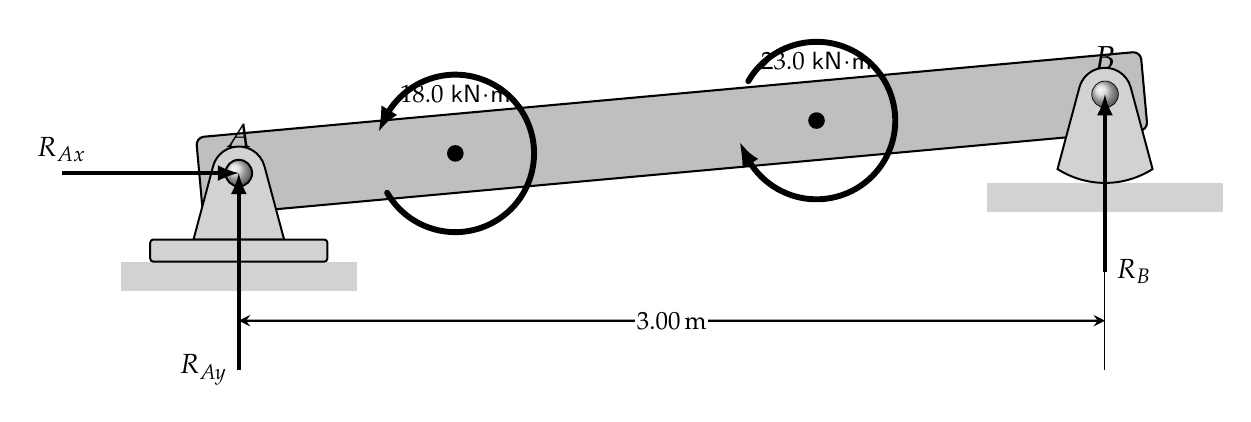
\begin{tikzpicture}[scale=\scale]
	\def\thickness{thick}
	\def\stroke{black}
	\def\hi{.4}
	\def\radii{0.5*\hi}
	\def\extend{3*\hi}
	\def\nuhi{0.45}
	\def\nuext{1.25}

	\coordinate (A) at (0, 0);
	\coordinate (D) at (11, 1);
	\coordinate (B) at ($ (A)!0.25!(D) $);
	\coordinate (C) at ($ (A)!0.667!(D) $);

	\fill[Gray!35] ($ (A)-(1.5,1.125) $) rectangle ($ (A)+(1.5,-1.5) $);
	\fill[Gray!35] ($ (D)-(1.5,1.125) $) rectangle ($ (D)+(1.5,-1.5) $);

	\Meme{A}{D}{Gray!50}{Gray!50}{black}{1}{0.1}{0.75}

	\fill[black] (A) circle (3pt) node[above, outer sep=2mm] {\large $A$};
	\fill[black] (B) circle (3pt) ;
	\fill[black] (C) circle (3pt);
	\fill[black] (D) circle (3pt) node[above, outer sep=2mm] {\large $B$};

	\PC{A}{Gray!35}{black}{1.125}{0.25}
	\Rocker{D}{Gray!35}{black}{1.125}{0.25}
	\Couple{B}{black}{1}{0.75}
	\Couple[0]{C}{black}{1}{0.75}

	\node[yshift=0.75cm] at (B) {\small $18.0\mathsf{\;kN\cd m}$};
	\node[yshift=0.75cm] at (C) {\small $23.0\mathsf{\;kN\cd m}$};

	% \draw[->, >=stealth, blue, ultra thick] ($ (B)+(60:0.875) $) node[black, above, outer sep=1mm]{\small $18.00\mathsf{\;kN\cdot m}$} arc (60:360:0.875)-- +(90:0.375);
	% \draw[->, >=stealth, blue, ultra thick] ($ (C)+(330:0.875) $) node[black, below, outer sep=3mm]{\small $23.0\mathsf{\;kN\cdot m}$} arc (330:30:0.875)-- +(-65:0.375);

	\draw ($ (A)+(0,-0.75) $) -- +(0,-1.752);
	\draw ($ (D)+(0,-0.75) $) --  +(0,-2.752);

	\draw[thick, <->, >=stealth] ([yshift=-1.875cm]A) -- node[fill=white, inner sep= 0.2mm]{\small $3.00\,$m}([yshift=-2.875cm]D);

	\draw[latex-,  ultra thick] (D) -- +(0,-2.25) node[right] {$R_{B}$};
	\draw[latex-,  ultra thick] (A) -- +(0,-2.5) node[left] {$R_{Ay}$};
	\draw[latex-,  ultra thick] (A) -- +(-2.25,0) node[above] {$R_{Ax}$};



\end{tikzpicture}

  }
\end{textblock*}


%%%%%%%%%%%%%%%%%%%%%%%%%%%%%%%%%%%%%%%%%%%%%%%%%%%%%%%%%%%%%%%%%%%%%%%%%%%%%%%%%%%%%%%%%%%%%%%%%%%%
% page 6 
%%%%%%%%%%%%%%%%%%%%%%%%%%%%%%%%%%%%%%%%%%%%%%%%%%%%%%%%%%%%%%%%%%%%%%%%%%%%%%%%%%%%%%%%%%%%%%%%%%%%
~\newpage
\begin{textblock*}{1.0\textwidth}(1in, 0.25in)
	
\begin{tikzpicture}[line width= 0.3mm, scale=1.0525]
		\draw[ color=gray!50, step=0.25in] (0,0) grid (7in,10in);
	\end{tikzpicture}
\end{textblock*}

\begin{textblock*}{3.255in}(1in, 0.1in)
	\cbox{
		\underbar{\bf Exercise 4:}\parm
		$ABCD$ has a negative couple applied at $B$ and is supported by a cable at $D$. 
			\begin{enumerate}
				\item Determine the magnitude of $T$ if $\Sigma M_A=0$.
				\item Determine the reaction at $A$ if $\Sigma F_x = \Sigma F_y =0$.				
			\end{enumerate}
	}
\end{textblock*}
\begin{textblock*}{3.125in}(4.775in, 0.1in)
  \cbox{
    \centering
    \def\scale{0.5}
    \input{../../pikz/05Moments/05Moments15Handout.tex}
  }
\end{textblock*}



\begin{textblock*}{2in}(1in, 5in)
	\cbox{
		\underbar{\bf Example 7:}\parm
		Determine the moment of the distributed load about  $O$.
	}
\end{textblock*}
\begin{textblock*}{4.35in}(3.55in, 5in)
  \cbox{
    \centering
    \def\scale{0.9}
    % !TEX root = ../../Beamer/05Moments/05Moments.tex


\makeatletter
\providecommand{\gettikzxy}[3]{%
	\tikz@scan@one@point\pgfutil@firstofone#1\relax
	\edef#2{\the\pgf@x}%
	\edef#3{\the\pgf@y}%
	}
	\makeatother

\tikz[scale=\scale]{
	\coordinate (A) at (-1,0);
	\coordinate (B) at (6,0);

	\def\hi{0.2}

	\coordinate (D) at (0,0.24);
	\coordinate (E) at (2,2.2);
	\coordinate (F) at (6,1.2);

	\gettikzxy{(A)}{\ax}{\ay};
	\gettikzxy{(D)}{\ddx}{\ddy};
	\gettikzxy{(E)}{\eex}{\eey};
	\gettikzxy{(B)}{\bbx}{\bby};

	\fill[top color=Gray!50, bottom color=Gray!30] (-2,-1.2) rectangle (6.75,-0.6);

	\Meme{A}{B}{Gray!50}{Gray!30}{black}{0.45}{0.225}{0.5}
	\PC{A}{Gray!50}{black}{0.6}{0.125};
	\Rocker{B}{Gray!50}{black}{0.6}{0.125};

	\DL{D}{E}{D}{gray!20}{black}{5}{0.35}{7}
	\DL{E}{F}{D}{gray!20}{black}{10}{0.35}{7}

	\node[above] at (E) {\small $3.00\thinspace\text{kN/m}$};
  \node[right] at (F) {\small $1.50\thinspace\text{kN/m}$};

	\draw (\ax,-0.25)--(\ax,-1.75);
	\draw (\ddx,0)--(\ddx,-1.75);
	\draw (\eex,0)--(\eex,-1.75);
	\draw (\bbx,-0.25)--(\bbx,-1.75);

	\node[yshift=0.42cm] at (A){$O$};


\footnotesize
	\draw[latex-latex] (\ax,-1.375) -- node[fill=white, inner sep=0]{$1.00\,\text{m}$}(\ddx,-1.375);
	\draw[latex-latex] (\ddx,-1.375) -- node[fill=white, inner sep=0.5mm]{$2.00\,\text{m}$}(\eex,-1.375);
	\draw[latex-latex] (\eex,-1.375) -- node[fill=white, inner sep=0.5mm]{$4.00\,\text{m}$}(\bbx,-1.375);


}

  }
\end{textblock*}



%%%%%%%%%%%%%%%%%%%%%%%%%%%%%%%%%%%%%%%%%%%%%%%%%%%%%%%%%%%%%%%%%%%%%%%%%%%%%%%%%%%%%%%%%%%%%%%%%%%%
% page 7
%%%%%%%%%%%%%%%%%%%%%%%%%%%%%%%%%%%%%%%%%%%%%%%%%%%%%%%%%%%%%%%%%%%%%%%%%%%%%%%%%%%%%%%%%%%%%%%%%%%%
~\newpage
\begin{textblock*}{1.0\textwidth}(1in, 0.25in)
	
\begin{tikzpicture}[line width= 0.3mm, scale=1.0525]
		\draw[ color=gray!50, step=0.25in] (0,0) grid (7in,10in);
	\end{tikzpicture}
\end{textblock*}

\begin{textblock*}{2in}(1in, 0.1in)
	\cbox{
		\underbar{\bf Exercise 5:}\parm
		Determine the moment of the distributed load about  $(0,0)$.
	}
\end{textblock*}
\begin{textblock*}{4.35in}(3.55in, 0.1in)
  \cbox{
    \centering
    \def\scale{1.25}
    % !TEX root = ../all/statikz.tex

\tikz[scale=\scale]{
  \coordinate (O) at (0,0);
  \coordinate (A) at (0,1);
  \coordinate (B) at (1.5,2.5);
  \coordinate (C) at (3,1.75);
  \coordinate (D) at (4.5,0);

  \DL{A}{B}{D}{Gray!20}{black}{5}{0.4}{6}
  \DL{B}{C}{D}{Gray!20}{black}{5}{0.4}{6}
  \DL{C}{D}{D}{Gray!20}{black}{5}{0.4}{6}

  \fill[Gray!50] (-1,-0.75) rectangle (5.5,0);
  \draw (-1,0) -- (5.5, 0);

  \node[black, above left] at (O) {\small $(0,0)$};
  \fill[black] (A) circle (1pt) node[black, above left] {\small $1.00\thinspace\text{kN/m}$};
  \fill[black] (B) circle (1pt) node[black, above right] {\small $2.50\thinspace\text{kN/m}$};
  \fill[black] (C) circle (1pt) node[black, above right] {\small $1.75\thinspace\text{kN/m}$};
  % \fill[Cornsilk3!50!black] (D) circle (1pt);

  \draw ($ (O)+(0,-0.125) $) -- +(0,-.5);
  \draw ($ (B)+(0,-2.625) $) -- +(0,-.5);
  \draw ($ (C)+(0,-1.875) $) -- +(0,-.5);
  \draw ($ (D)+(0,-0.125) $) -- +(0,-.5);

  \draw[latex-latex] ($ (O)+(0,-0.375) $) -- node[fill=Gray!50] {\small $1.50\thinspace\text{m}$}($ (B)+(0,-2.875) $);
  \draw[latex-latex] ($ (B)+(0,-2.875) $) --  node[fill=Gray!50] {\small $1.50\thinspace\text{m}$}($ (C)+(0,-2.125) $);
  \draw[latex-latex] ($ (C)+(0,-2.125) $) --  node[fill=Gray!50] {\small $1.50\thinspace\text{m}$}($ (D)+(0,-0.375) $);
}

  }
\end{textblock*}


\end{document}